\documentclass[9pt,twocolumn,twoside]{styles/osajnl}
\usepackage{fancyvrb}
\journal{i524} 

\title{ On-line advertisement click prediction}

\author[1,*]{Sahiti Korrapati}

\affil[1]{School of Informatics and Computing, Bloomington, IN 47408, U.S.A.}

\affil[*]{Corresponding authors: sakorrap@iu.edu, S17-IR-2013}

\dates{March 13, 2017}

\ociscodes{Hadoop, Ad click Prediction, BigData, Ansible, Chameleon cloud}

% replace this with your url in github/gitlab
\doi{\url{https://github.com/sakorrap/sp17-i524/tree/master/project/S17-IR-2013/report.pdf}}

\begin{abstract}
This project aims at predicting the most suitable advertisements to be displayed on the web pages based on relevance by ranking each ad based on the liklihood of clicking. Data is obtained as CSV files from Kaggle Datasets and is stored in Hadoop Data File system(HDFS). In this project, various Bigdata tools and softwares are used to carry out the analytical computations efficiently. And Ansible is used to deploy all the necessary softwares on a cloud.
\newline
\end{abstract}

\setboolean{displaycopyright}{true}

\begin{document}

\maketitle

\section{Introduction}
It has been analyzed that an average American spends about 23 hours per week surfing on-line \cite{news-social-media}. This on-line user activity is being captured by companies to perform analysis for advertisements or recommendations or any other purpose. This has given rise to the field of "Web Analytics" and one such application is Ad Click prediction.
Many measures are available to assess the ad performance. One such measure to assess the immediate ad response is click-through rate (CTR) of the advertisement \cite{dictionary-clickThrough} which is defined as the ratio of a number of clicks on an ad to the number of times the ad is shown, expressed as a percentage \cite{wiki-clickThrough}.
The user activity data that is used for prediction is enormous. To handle such large volumes of data Big data technologies come handy. The dataset that we are dealing with in this project is released by Outbrain which is 2 Billion page views and 16,900,000 clicks of 700 Million unique users, across 560 sites \cite{kaggle-outbrain}. The data is anonymized and is in CSV file format. Paraquet compressing along with impala/drill to be decided to query and analyze the data compressed in files that are stored in HDFS. Programming language for analyzing the data is yet to be decided between JAVA and Python. Ansible is used to deploy the software and chameleon cloud for running virtual machines.

\section{Background}
The dataset contains a sample of users’ page views and clicks, as observed on multiple publisher sites in the United States between 14-June-2016 and 28-June-2016. Each viewed page or clicked recommendation is further accompanied by some semantic attributes of those documents \cite{kaggle-outbrain}.
The dataset contains numerous sets of content recommendations served to a specific user in a specific context. Each context (i.e. a set of recommendations) is given a display\_id. In each such set, the user has clicked on at least one recommendation. Our task is to rank the recommendations in each group by decreasing predicted likelihood of being clicked \cite{kaggle-outbrain}.

\subsection{Data fields description}
Each user in the dataset is represented by a unique id (uuid). A person can view a document (document\_id), which is simply a web page with content (e.g.  a news article). On each document, a set of ads (ad\_id) are displayed. Each ad belongs to a campaign (campaign\_id) run by an advertiser (advertiser\_id). Figure \ref{fig:OutbrainData} shows the fields in our dataset. Metadata about the document is also provided, such as which entities are mentioned, a taxonomy of categories, the topics mentioned, and the publisher \cite{kaggle-outbrain}.

\begin{figure}[htbp]
\centering
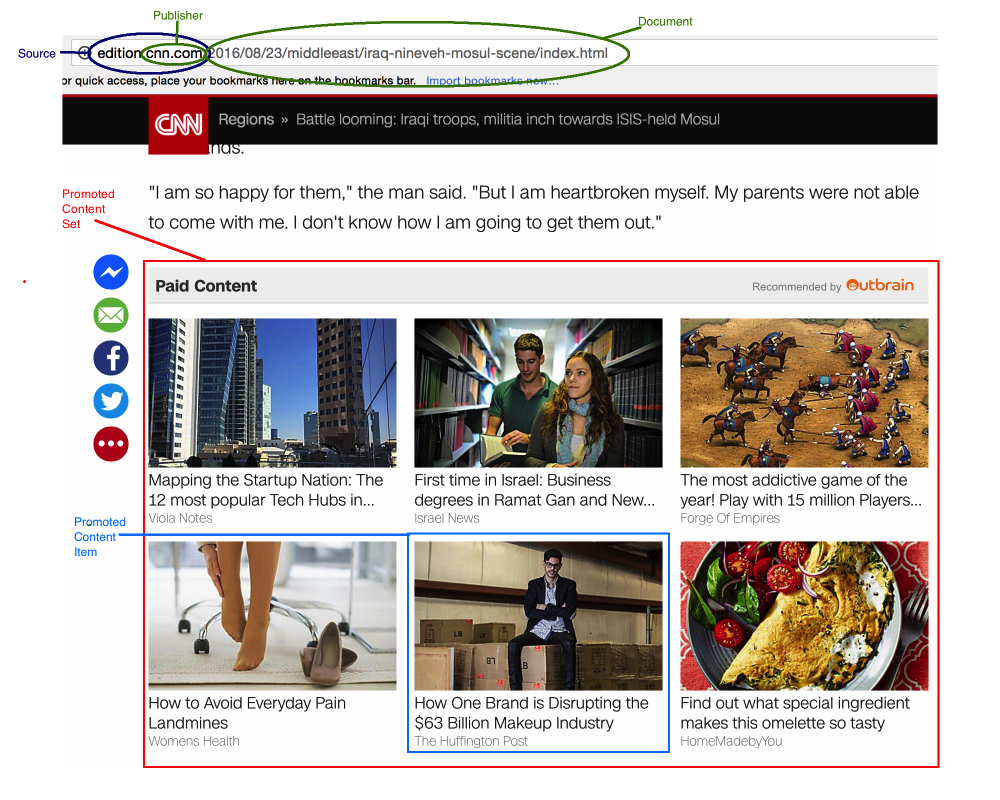
\includegraphics[width=\linewidth]{images/page_view.png}
\caption{Displaying Source, Publisher, Document, Promoted content set and items \cite{kaggle-outbrain}}
\label{fig:OutbrainData}
\end{figure}

\section{Setup and Configuration}
TBD

\section{Work Flow}
TBD

\section{Experiments and Results}
TBD

\section{Licensing}
TBD

\section{Conclusion}
% Due on April 17
TBD

\section{Execution Summary}
\begin{enumerate}
    \item{Feb 23 - Mar 6, 2017} Exploring Python, Ansible and Chameleon cloud
    \item{Mar 10 - Mar 13, 2017} Exploring the datasets available and come up with the project proposal
    \item{Mar 14 - Mar 20, 2017} Decide on the architecture and workflow
    \item{Mar 21 - Mar 24, 2017} Configure and setup the workbench
    \item{Mar 25 - Mar 30, 2017} Prepare high level design
    \item{Mar 31 - Apr 6, 2017} Implementation and Testing
    \item{Apr 7 - Apr 11, 2017} Automate the deployment process using Ansible
    \item{Apr 12 - Apr 17, 2017} Optimizing and work on benchmarking
    \item{Apr 18 - Apr 22, 2017} Project review and completing any pending work
    \item{Apr 23 - Apr 24} Complete the report and commit the code
\end{enumerate}

\section*{Acknowledgements}

The authors thank Professor Gregor Von Laszewski and all the AIs of big data class for the guidance and technical support.

% Bibliography
\bibliography{references}
 
\section*{Author Biographies}
\begingroup
\setlength\intextsep{0pt}
\begin{minipage}[t][3.2cm][t]{1.0\columnwidth} % Adjust height [3.2cm] as required for separation of bio photos.
  \noindent
  {\bfseries Sahiti Korrapati} is pursuing her MSc in Data Science from
  Indiana University Bloomington
\end{minipage}
\endgroup
\end{document}
